\section*{Pág 60 - 5}
\subsection*{A}
\begin{lstlisting}[mathescape]
$\int_{1}^{2}\frac{k}{x} = 1$

$k \int_{1}^{2}\frac{1}{x} = 1$

$k[Lnx |^2_1] = 1$

$k[ln2 - ln1] = 1$

$k * ln2 = 1$

$k = \frac{1}{ln2} = 1,44$
\end{lstlisting}

\subsection*{B}
\begin{lstlisting}[mathescape]
$f(x) = \frac{1,44}{x}$
$\mu (x) = \int^2_1 x * \frac{1,44}{x}dx$
$\mu (x) = 1,44x|^2_1 = 1,44 * 2 - 1,44 * 1 = 1,44$
\end{lstlisting}

\subsection*{C}
\begin{lstlisting}[mathescape]
$F(md) = 0,5 = \int^{md}_1 \frac{1,44}{x}dx$
$0,5 = 1,44[Lnmd - Ln1]$
$0,5 = 1,44Lnmd$
$Lnmd = \frac{0,5}{1,44}$
$md = e^{\frac{0,5}{1,44}} = e^{0,35} = 1,42$
\end{lstlisting}

\subsection*{D}
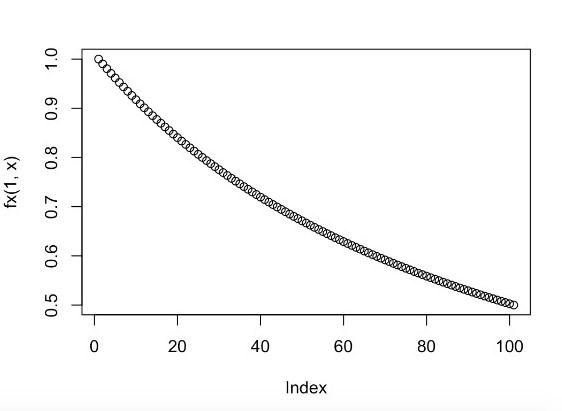
\includegraphics[width=\textwidth]{P60_05_D.jpeg}

\subsection*{E}
\begin{lstlisting}[mathescape]
$\sigma^2 = \int^2_1 (x - 1,44)^2 \frac{1,44}{x}dx$
$= 1,44 \int^2_1 (x - 2,88 + \frac{1,44^2}{x})$
$= 1,44 [\frac{x^2}{2}|^2_1 - 2,88x|^2_1 + 1,44^2lnx|^2_1]$
$= 1,44 [(2 - \frac{1}{2}) - 2,88 + 1,44^2ln2] = 0,08$
\end{lstlisting}
